% Don't touch this %%%%%%%%%%%%%%%%%%%%%%%%%%%%%%%%%%%%%%%%%%%
\documentclass[12pt]{article}
\usepackage{fullpage}
\usepackage[left=1in,top=1in,right=1in,bottom=1in,headheight=3ex,headsep=3ex]{geometry}
\usepackage{graphicx}
\usepackage{float}
\usepackage{array}


\newcommand{\blankline}{\quad\pagebreak[2]}
%%%%%%%%%%%%%%%%%%%%%%%%%%%%%%%%%%%%%%%%%%%%%%%%%%%%%%%%%%%%%%

% Modify Course title, instructor name, semester here %%%%%%%%

\title{PHY115: Final Exam}
\author{Spring 2021}
\date{}

%%%%%%%%%%%%%%%%%%%%%%%%%%%%%%%%%%%%%%%%%%%%%%%%%%%%%%%%%%%%%%

% Don't touch this %%%%%%%%%%%%%%%%%%%%%%%%%%%%%%%%%%%%%%%%%%%
\usepackage[sc]{mathpazo}
%\linespread{1.05} % Palatino needs more leading (space between lines)
\usepackage[T1]{fontenc}
\usepackage[mmddyyyy]{datetime}% http://ctan.org/pkg/datetime
\usepackage{advdate}% http://ctan.org/pkg/advdate
\newdateformat{syldate}{\twodigit{\THEMONTH}/\twodigit{\THEDAY}}
\newsavebox{\MONDAY}\savebox{\MONDAY}{Mon}% Mon
\newcommand{\week}[1]{%
%  \cleardate{mydate}% Clear date
% \newdate{mydate}{\the\day}{\the\month}{\the\year}% Store date
  \paragraph*{\kern-2ex\quad #1, \syldate{\today} - \AdvanceDate[4]\syldate{\today}:}% Set heading  \quad #1
%  \setbox1=\hbox{\shortdayofweekname{\getdateday{mydate}}{\getdatemonth{mydate}}{\getdateyear{mydate}}}%
  \ifdim\wd1=\wd\MONDAY
    \AdvanceDate[7]
  \else
    \AdvanceDate[7]
  \fi%
}
%\usepackage{setspace}
\usepackage{multicol}
%\usepackage{indentfirst}
\usepackage{fancyhdr,lastpage}
\usepackage{url}
\pagestyle{fancy}
\usepackage{hyperref}
\usepackage{lastpage}
\usepackage{amsmath}
\usepackage{layout}

\lhead{}
\chead{}
%%%%%%%%%%%%%%%%%%%%%%%%%%%%%%%%%%%%%%%%%%%%%%%%%%%%%%%%%%%%%%

% Modify header here %%%%%%%%%%%%%%%%%%%%%%%%%%%%%%%%%%%%%%%%%
%\rhead{\footnotesize Text in header}

%%%%%%%%%%%%%%%%%%%%%%%%%%%%%%%%%%%%%%%%%%%%%%%%%%%%%%%%%%%%%%
% Don't touch this %%%%%%%%%%%%%%%%%%%%%%%%%%%%%%%%%%%%%%%%%%%
\lfoot{}
\cfoot{\small \thepage/\pageref*{LastPage}}
\rfoot{}

\usepackage{array, xcolor}
\usepackage{color,hyperref}
\definecolor{clemsonorange}{HTML}{EA6A20}
\hypersetup{colorlinks,breaklinks,linkcolor=clemsonorange,urlcolor=clemsonorange,anchorcolor=clemsonorange,citecolor=black}

\begin{document}

\maketitle

%\blankline

%\begin{tabular*}{.93\textwidth}{@{\extracolsep{\fill}}lr}

%%%%%%%%%%%%%%%%%%%%%%%%%%%%%%%%%%%%%%%%%%%%%%%%%%%%%%%%%%%%%%


\begin{center}
 Deadline:  Wednesday the 21th
\end{center}
\hrule



% First Section %%%%%%%%%%%%%%%%%%%%%%%%%%%%%%%%%%%%%%%%%%%%
\section*{Theory Questions (30 p)}

\begin{enumerate}
    \item Newton's Laws
    \begin{itemize}
        \item When are Newton's Laws valid?
        \item Can you use the second Law of Newton to explain the first one? How?
        \item Is the normal force the reaction pair of the weight? Why not? or why yes?
    \end{itemize}
    
    \item Linear Momentum
\begin{itemize}
    \item Define Linear Momentum.
    \item Write the 2nd Law of Newton in terms of the linear momentum.
    \item When is the linear momentum conserved?
    \item When is a component conserved?
    \item Give an example in which the linear momentum is not conserved, 
    but one of its coordinates is. 
    \item EXTRA CREDIT (5 p): Find a scene on a Movie or in your animation short to illustrate the previous point, attach the link to the scene.
\end{itemize}
\item Angular Momentum
\begin{itemize}
    \item Define Torque and Angular Momentum.
    \item Write the equation that relates the angular momentum and torque.
    \item Write the equation for Angular Momentum that is equivalent to the definition of  Linear Momentum.
    \item Write the equation for Torque that is equivalent to the 2nd Law of Newton.
    \item When is the Angular Momentum conserved?
    \item Give an example in which the Angular Momentum is conserved.
    \item EXTRA CREDIT (5 p): Find a scene on a Movie or in your animation short to illustrate the previous point, attach the link to the scene.
\end{itemize}
\end{enumerate}

\section*{Test your undertanding (20 p)}
\vspace{7mm}


\begin{enumerate}
    \item A helicopter has a large main rotor that rotates in a horizontal
    plane and provides lift. There is also a small rotor on the tail
    that rotates in a vertical plane. What is the purpose of the tail rotor?
    (Hint: If there were no tail rotor, what would happen when the
    pilot changed the angular speed of the main rotor?).
    \item A bullet spins on its axis as it emerges from a rifle. Explain
    how this prevents the bullet from tumbling and keeps the streamlined
    end pointed forward.
    \item A  client brings a treasured ball to your engineering
    firm, wanting to know whether the ball is solid or hollow. 
    Design a simple, inexpensive experiment that you could perform
    quickly, without injuring the precious ball, to find out whether it is
    solid or hollow.
  
\end{enumerate}

\section*{Exercises (50 p)}
\vspace{7mm}

\section*{1: Billiard Physics}

A cue ball (a uniform solid sphere of mass $m$ and radius $R$) is at
rest on a level pool table. Using a pool cue, you give the ball a
sharp, horizontal hit of magnitude $F$ at different heights (see figure \ref{fig:1} panels a-d)
In panel (a) $h$ is defined so that the ball will roll without slipping. In panel (b), the hit height is higher than $h$. In panel (c) the hit is right in the center of the ball, and in panel (d) the hit height is lower than
$h$. 
\begin{itemize}
    \item In panels 1-4 of the figure \ref{fig:1}, we can observe how the ball will move after the hit. Match each one of the panels a-d with the corresponding motion after the hit shown in panels 1-4.
    \item What is the acceleration of the center of mass after the hit in terms of the friction force and $m$?
    \item What is the torque after the hit in terms of the friction force and $R$?
\end{itemize}


\begin{figure}[h!]
  \centering
  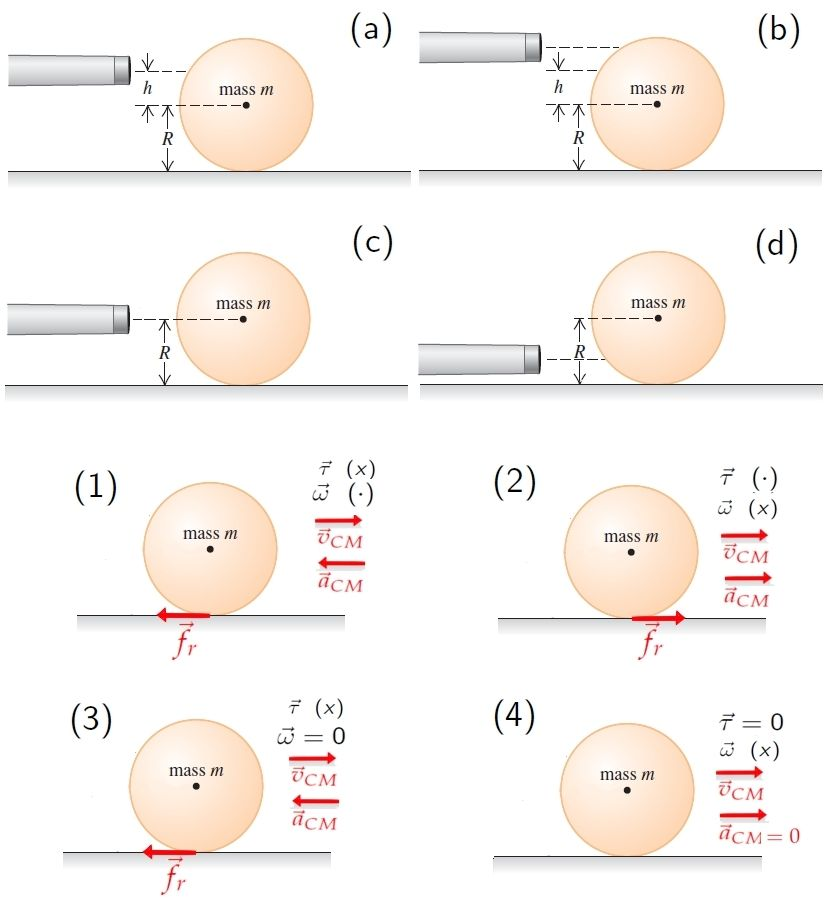
\includegraphics[width=1.\textwidth]{images/ball_a.jpg}
  \caption{Panels (a) to (d): $h$ is defined so that the ball will roll without slipping. In panel (b), the hit 
  height is higer than $h$. In panel (c) the hit is right in the center of the ball, and in panel (d) the hit height is bellow. Panels (1) to (4): motion after the hit .}
  \label{fig:1}
\end{figure}

\vspace{14mm}

\newpage



\section*{2: Elastic Collision}

 Consider a ball that bounces with a wall on a horizontal surface without friction. If the collision is elastic,
the kinetic energy of the ball is conserved, and the magnitude of the linear momentum after the collision is equal to the initial:
\begin{equation}
    |\vec{p}_f|=|\vec{p}_i|
\end{equation}
Proof that the initial angle ($\theta_i$) is equal to the final angle ($\theta_f$). 
\vspace{7mm}



\begin{figure}[h!]
  \centering
  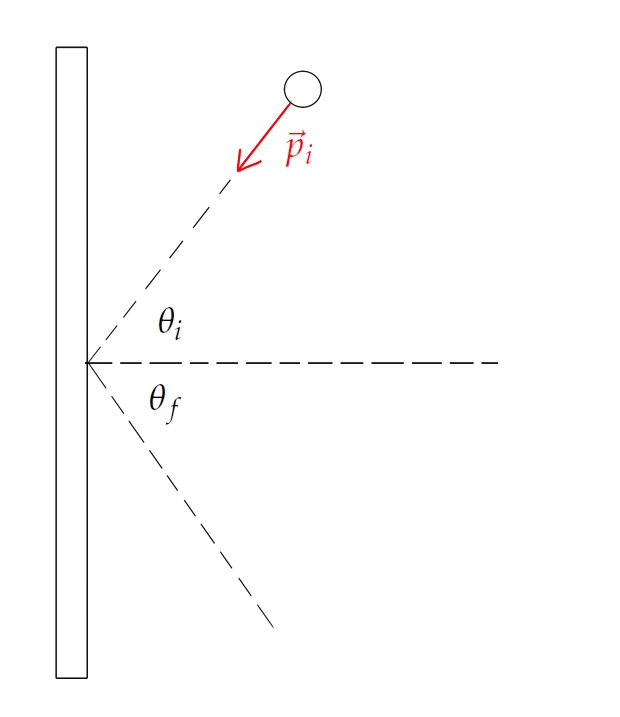
\includegraphics[width=0.6\textwidth]{images/collision.jpg}
  \caption{ Ball bouncing  with a wall in an horizontal surface without friction.}
  \label{fig:3}
\end{figure}


Hint= Which component of $\vec{p}$ is conserved? 

\newpage

\section*{3: Light and materials}

Find and explain the difference in the parameters for the materials shown in the figure \ref{fig:3}. 

\begin{figure}[h!]
    \centering
    \includegraphics[width=0.9\textwidth]{images/materials.jpg}
    \caption{Interaction of light with a metal (top panel) and a non-metallic material (lower panel).}
    \label{fig:4}
  \end{figure}



\end{document}


